\chapter{Logam: Reaksi dengan Asam dan Korosi}\label{ch:g9:metals-acids-corrosion}

Di sebuah pelabuhan, lambung baja sebuah kapal nelayan tua bergaris-garis
\omterm{def:g9:metals-acids-corrosion:corrosion}{karat} jingga. Di dermaga, sebuah pagar berlapis seng telah berdiri di
bawah hujan selama tiga puluh tahun dan masih berkilau kelabu kusam. Di
sebuah museum, sebentuk cincin emas yang terkubur selama tiga ribu tahun
masih secemerlang hari ketika cincin itu dibuat. Logam-logam tidak
semuanya menghadapi dunia dengan cara yang sama: sebagian diserang air,
\omterm{def:g4:air-a-mixture-of-gases:air}{udara}, dan asam, sebagian lagi hampir tidak sama sekali.

\begin{recall}
\omterm{def:g9:ions:ion}{Ion} adalah \omterm{def:g7:atoms-and-molecules:atom}{atom} yang bermuatan; logam membentuk \omterm{def:g9:ions:ion}{kation} seperti
\ce{Fe^{2+}}, \ce{Zn^{2+}}, \ce{Al^{3+}}, yang dikenali dengan uji
\omterm{def:g3:separating-mixtures:decant}{pengendapan} (\cref{ch:g9:ions}). \omterm{def:g9:acids-bases-ph:acidic}{Larutan asam} mengandung banyak \omterm{def:g9:ions:ion}{ion}
\ce{H+(aq)} (\cref{ch:g9:acids-bases-ph}). Hidrogen \omterm{def:g4:what-a-fire-needs:burning}{terbakar} dengan
letupan melengking di mulut tabung reaksi
(\cref{ch:g7:identifying-substances}).
\end{recall}

\begin{omfigure}
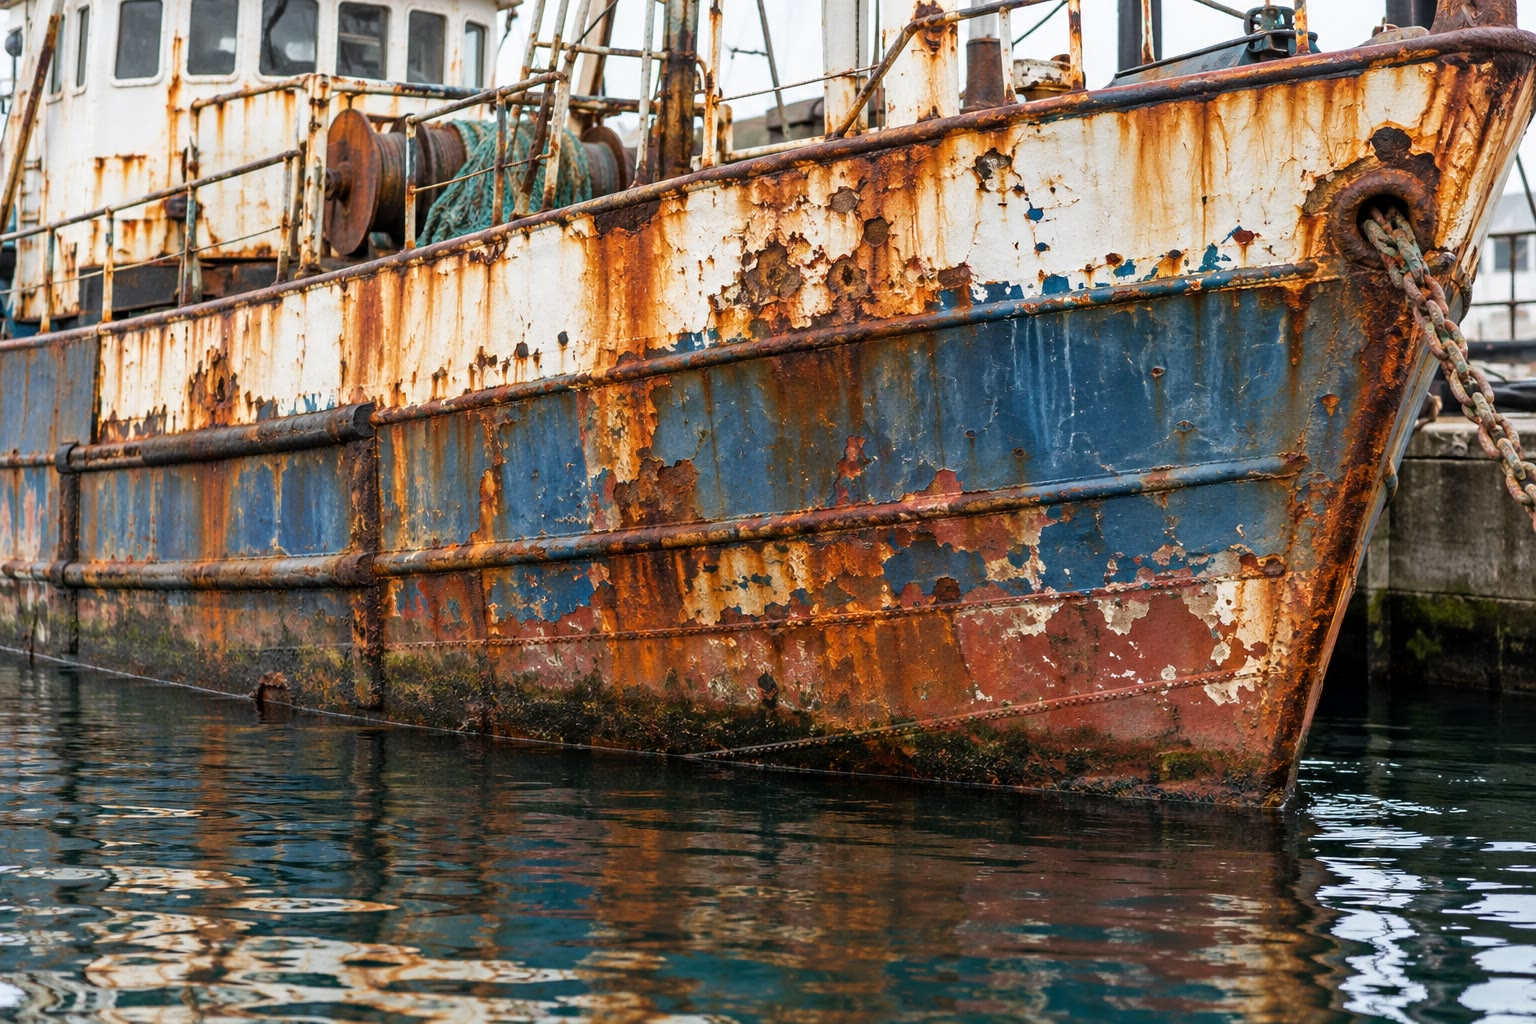
\includegraphics[width=0.55\linewidth]{images/book1/ai/g9-rusty-hull.jpg}

{\small Lambung kapal tua: bajanya sedang berkarat.}
\end{omfigure}

\section{Logam dalam asam klorida}

\begin{inthelab}[Tiga logam dalam asam]
Guru menjatuhkan sepotong kecil besi, seng, dan tembaga ke dalam tiga
tabung reaksi berisi asam klorida encer. Gelembung-gelembung naik dari
besi dan seng, perlahan dari besi, deras dari seng, dan logam-logam itu
perlahan menghilang; tidak terjadi apa-apa pada tembaga. Gas yang
ditampung dalam tabung kecil menimbulkan letupan melengking: gas itu
hidrogen. Dengan natrium hidroksida, cairan tabung pertama memberikan
\omterm{def:g9:ions:precipitate}{endapan} hijau (\omterm{def:g9:ions:ion}{ion} \ce{Fe^{2+}}), cairan tabung kedua \omterm{def:g9:ions:precipitate}{endapan} putih (\omterm{def:g9:ions:ion}{ion}
\ce{Zn^{2+}}).
\end{inthelab}

\begin{omfigure}
\begin{tikzpicture}[font=\small, scale=1.2]
  \foreach \k/\m/\c/\bub in {0/besi/black!45/4, 1/seng/black!25/9, 2/tembaga/orange!60!brown/0} {
    \pic[transform shape] at (\k*2.4,0) {testtube={0.55}{omWater!70}};
    \fill[\c] (\k*2.4-0.13,0.08) rectangle (\k*2.4+0.13,0.35);
    \ifnum\bub>0
      \foreach \j in {1,...,\bub} {
        \pgfmathsetmacro\yy{0.45+0.12*\j}
        \pgfmathsetmacro\xx{\k*2.4+0.1*sin(97*\j)}
        \draw[black!55] (\xx,\yy) circle (0.035);
      }
    \fi
    \node[anchor=north, align=center] at (\k*2.4,-0.15) {\m};
  }
  \node[anchor=north, align=center, font=\footnotesize] at (0,-0.6) {bergelembung, pelan};
  \node[anchor=north, align=center, font=\footnotesize] at (2.4,-0.6) {bergelembung, deras};
  \node[anchor=north, align=center, font=\footnotesize] at (4.8,-0.6) {tidak bereaksi};
\end{tikzpicture}

{\small Besi, seng, dan tembaga dalam asam klorida encer: besi dan seng
melepaskan hidrogen; tembaga tidak bereaksi.}
\end{omfigure}

\begin{proposition}[Logam ditambah asam]\label{prop:g9:metals-acids-corrosion:acid}
Banyak logam --- besi, seng, aluminium, magnesium --- bereaksi dengan
\omterm{def:g9:ions:ion}{ion-ion} \ce{H+} sebuah asam: logam itu menghilang sebagai \omterm{def:g9:ions:ion}{ion-ion} logam,
yang tetap terlarut, dan gas hidrogen dilepaskan. Tembaga, perak, dan
emas tidak bereaksi dengan asam klorida.
\end{proposition}

\section{Menuliskan persamaan dengan ion}

\begin{definition}[Ion penonton]\label{def:g9:metals-acids-corrosion:spectator}
\omterm{def:g9:ions:ion}{Ion} yang ada di dalam larutan selama reaksi berlangsung tetapi tidak
ikut bereaksi, dan ditemukan tanpa berubah di akhir reaksi, disebut
\emph{ion penonton}\index{ion penonton}. \omterm{def:g9:ions:ion}{Ion} itu tidak dituliskan dalam
persamaan.
\end{definition}

\begin{example}[Besi dan seng dalam asam klorida]\label{ex:g9:metals-acids-corrosion:iron}
Asam klorida mengandung \omterm{def:g9:ions:ion}{ion} \ce{H+(aq)} dan \ce{Cl-(aq)}. \omterm{def:g9:ions:ion}{Ion-ion} klorida
ditemukan tanpa berubah di akhir reaksi: \omterm{def:g9:ions:ion}{ion-ion} itu penonton.
Persamaannya adalah
\[
  \ce{Fe(s) + 2H+(aq) -> Fe^{2+}(aq) + H2(g)}, \qquad
  \ce{Zn(s) + 2H+(aq) -> Zn^{2+}(aq) + H2(g)}.
\]
Keduanya setara baik \omterm{def:g7:atoms-and-molecules:atom}{atomnya} maupun muatannya: $+2$ di setiap ruas.
\end{example}

\begin{method}[Menuliskan persamaan reaksi logam dengan asam]\label{met:g9:metals-acids-corrosion:write}
\begin{enumerate}
  \item \omterm{def:g7:chemical-reactions:reactant}{Pereaksi}: logam (s) dan \omterm{def:g9:ions:ion}{ion-ion} \ce{H+(aq)}.
  \item Produk: \omterm{def:g9:ions:ion}{ion} logam (aq), dengan muatannya yang biasa, dan
        hidrogen \ce{H2(g)}.
  \item Setarakan \omterm{def:g7:atoms-and-molecules:atom}{atom-atomnya}, lalu periksalah bahwa muatan totalnya
        sama di kedua ruas.
\end{enumerate}
Untuk aluminium: \ce{2Al(s) + 6H+(aq) -> 2Al^{3+}(aq) + 3H2(g)}; muatan
$+6$ di setiap ruas.
\end{method}

\begin{safety}{\ghs[0.8cm]{GHS02}\ghs[0.8cm]{GHS04}}
% ledger: ghs:H2
Hidrogen yang dilepaskan sangat mudah menyala. Reaksinya dilakukan dalam
tabung reaksi kecil, oleh guru, jauh dari nyala api apa pun kecuali
nyala yang dipakai untuk uji letupan.
\end{safety}

\section{Korosi}

\begin{definition}[Korosi dan karat]\label{def:g9:metals-acids-corrosion:corrosion}
Yang disebut \emph{korosi}\index{korosi} adalah serangan perlahan
terhadap sebuah logam oleh zat-zat di sekitarnya --- oksigen, air,
asam, garam --- yang mengubah logam itu menjadi \omterm{def:g9:ions:ion}{ion} atau senyawa
seperti oksida. Korosi besi dan baja menghasilkan
\emph{karat}\index{karat}, oksida besi terhidrasi yang cokelat dan
rapuh, yang mengelupas dan membiarkan serangan itu berlanjut lebih
dalam.
\end{definition}

\begin{proposition}[Yang diperlukan besi untuk berkarat]\label{prop:g9:metals-acids-corrosion:needs}
Besi hanya berkarat jika oksigen dan air sama-sama mencapainya. Garam
yang \omterm{def:g2:mixing-and-dissolving:dissolve}{larut} dalam air, seperti di jalan-jalan yang ditaburi garam pada
musim dingin atau di tepi laut, mempercepat perkaratan.
\end{proposition}

\begin{inthelab}[Tiga paku, satu minggu]
Tiga paku besi yang bersih ditempatkan dalam tiga tabung reaksi: yang
pertama dalam \omterm{def:g4:air-a-mixture-of-gases:air}{udara} kering bersama zat pengering yang menyerap uap air;
yang kedua dalam air yang telah dididihkan untuk menghilangkan \omterm{def:g4:air-a-mixture-of-gases:air}{udara}
terlarutnya, ditutup selapis minyak; yang ketiga separuh dalam air
keran, separuh di \omterm{def:g4:air-a-mixture-of-gases:air}{udara}. Seminggu kemudian, hanya paku ketiga yang
berkarat.
\end{inthelab}

\begin{omfigure}
\begin{tikzpicture}[font=\small, scale=1.2]
  % tube 1: dry air, drying agent
  \pic[transform shape] at (0,0) {testtube={0.18}{white!80!black}};
  \foreach \x/\y in {-0.12/0.15,0.08/0.12,-0.02/0.3,0.12/0.32,-0.14/0.42,0.03/0.48}
    \fill[black!35] (\x,\y) circle (0.05);
  \fill[black!45] (-0.03,1.0) rectangle (0.03,2.4);
  \fill[black!45] (-0.09,2.4) rectangle (0.09,2.48);
  \fill[black!60] (-0.3,2.8) rectangle (0.3,3.1);
  \node[anchor=north, align=center] at (0,-0.15) {udara kering:\\ tidak berkarat};
  % tube 2: boiled water under oil
  \pic[transform shape] at (2.6,0) {testtube={0.7}{omWater!80}};
  \fill[yellow!55!orange!60] (2.36,1.85) rectangle (2.84,2.1);
  \fill[black!45] (2.57,0.3) rectangle (2.63,1.7);
  \fill[black!45] (2.51,1.7) rectangle (2.69,1.78);
  \fill[black!60] (2.3,2.8) rectangle (2.9,3.1);
  \node[anchor=north, align=center] at (2.6,-0.15) {air tanpa udara:\\ tidak berkarat};
  % tube 3: water and air
  \pic[transform shape] at (5.2,0) {testtube={0.4}{omWater!80}};
  \fill[black!45] (5.17,0.3) rectangle (5.23,2.2);
  \fill[black!45] (5.11,2.2) rectangle (5.29,2.28);
  \fill[orange!60!brown] (5.15,0.9) rectangle (5.25,1.5);
  \node[anchor=north, align=center] at (5.2,-0.15) {air dan udara:\\ berkarat};
  \draw[<-, omProp, thick] (-0.15,0.3) -- (-0.9,0.7) node[left, text=black, font=\footnotesize] {zat pengering};
  \draw[<-, omProp, thick] (2.85,1.98) -- (3.6,2.4) node[right, text=black, font=\footnotesize] {minyak};
\end{tikzpicture}

{\small Percobaan tiga paku: besi hanya berkarat di tempat air dan
oksigen mencapainya bersama-sama, di sini di permukaan air.}
\end{omfigure}

\begin{example}[Aluminium dan tembaga melindungi dirinya sendiri]\label{ex:g9:metals-acids-corrosion:protect}
Aluminium langsung diserang oksigen \omterm{def:g4:air-a-mixture-of-gases:air}{udara}, tetapi lapisan tipis oksida
yang terbentuk melekat pada logam itu dan menutupinya dari \omterm{def:g4:air-a-mixture-of-gases:air}{udara}: kusen
jendela aluminium tahan puluhan tahun. Tembaga, yang perlahan diserang
\omterm{def:g4:air-a-mixture-of-gases:air}{udara}, air, dan karbon dioksida, menjadi tertutup kerak hijau, yaitu
patina, yang juga melekat dan melindungi logam di bawahnya. Sebaliknya,
\omterm{def:g9:metals-acids-corrosion:corrosion}{karat} mengelupas.
\end{example}

\begin{omfigure}
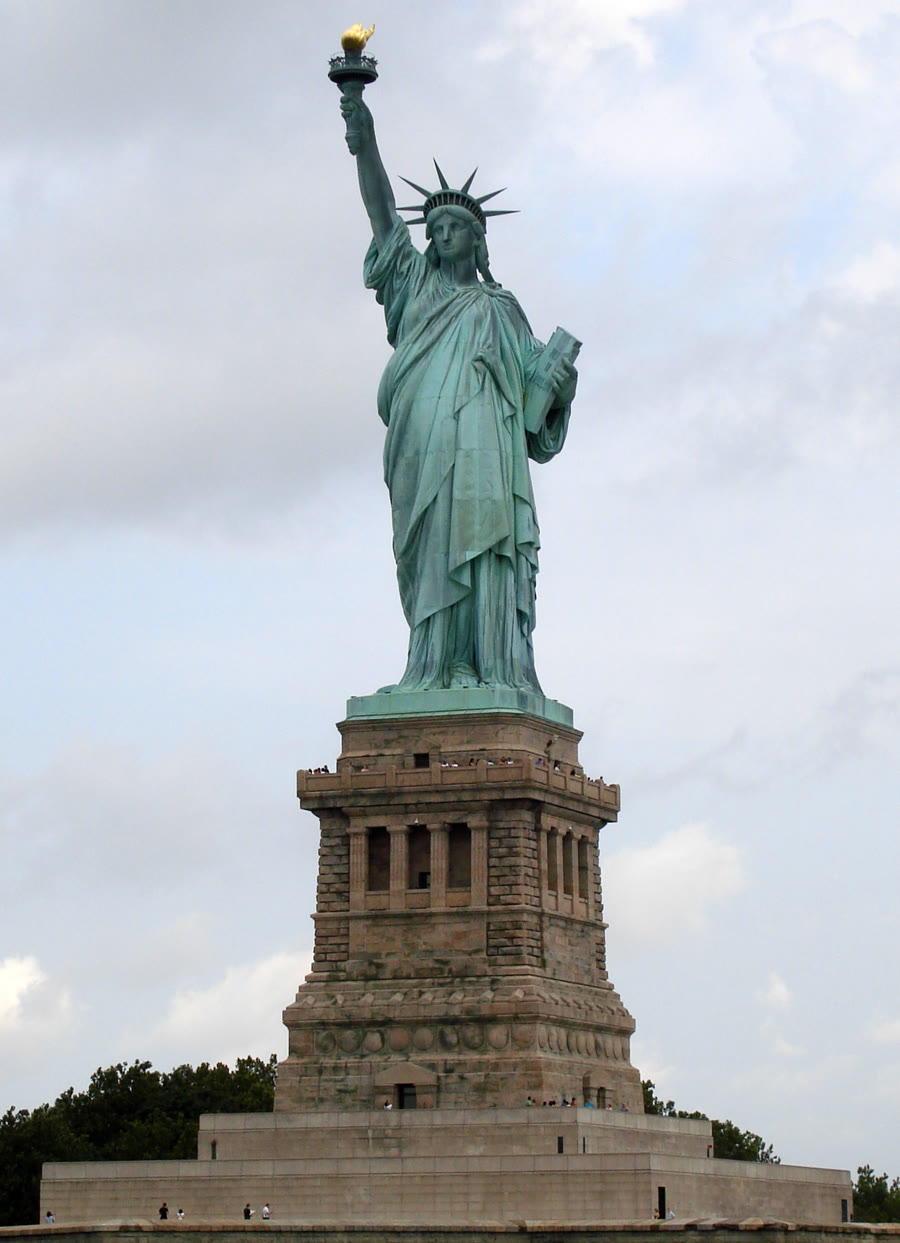
\includegraphics[height=6cm]{images/book1/statue-patina.jpg}

{\small Patung Liberty: kulit tembaganya tertutup patina hijau. Foto:
Elcobbola, domain publik.}
\end{omfigure}

\section{Melindungi logam}

\begin{definition}[Galvanisasi]\label{def:g9:metals-acids-corrosion:galvanising}
Yang disebut \emph{galvanisasi}\index{galvanisasi} adalah melapisi baja
dengan selapis seng, dengan mencelupkannya ke dalam seng cair. Seng
diserang \omterm{def:g4:air-a-mixture-of-gases:air}{udara} dan air menggantikan baja di bawahnya: bahkan di tempat
lapisan itu tergores, seng di dekatnya terkorosi lebih dulu dan bajanya
terhindar.
\end{definition}

\begin{proposition}[Cara melindungi besi dan baja]\label{prop:g9:metals-acids-corrosion:ways}
\begin{itemize}
  \item jauhkan air dan \omterm{def:g4:air-a-mixture-of-gases:air}{udara}: cat, minyak, gemuk, lapisan \omterm{def:g8:plastics:plastic}{plastik};
  \item \omterm{def:g9:metals-acids-corrosion:galvanising}{galvanisasi}: lapisan seng yang terkorosi menggantikan baja;
  \item pakailah baja tahan \omterm{def:g9:metals-acids-corrosion:corrosion}{karat}, paduan besi dengan kromium, yang
        melindungi dirinya dengan lapisan oksida tipis yang menutup
        rapat;
  \item pasang balok-balok seng pada lambung kapal: sengnya perlahan
        termakan menggantikan baja, dan diganti dari waktu ke waktu (cara
        kerjanya dijelaskan di salah satu buku universitas).
\end{itemize}
\end{proposition}

\begin{omfigure}
\begin{minipage}[b]{0.52\linewidth}\centering
\begin{tikzpicture}[font=\small]
  \fill[black!35] (0,0) rectangle (5,0.8);
  \fill[black!15] (0,0.8) rectangle (2.2,1.1);
  \fill[black!15] (2.8,0.8) rectangle (5,1.1);
  \fill[omWater!80] (1.6,1.1) rectangle (3.4,1.35);
  \fill[omWater!80] (2.2,0.8) rectangle (2.8,1.1);
  \draw[black!60] (0,0) rectangle (5,0.8);
  \foreach \x in {1.95,2.1} \draw[->, omProp, thick] (\x,1.25) -- (\x+0.05,1.7);
  \node[anchor=west, font=\footnotesize] at (5.1,0.4) {baja};
  \node[anchor=west, font=\footnotesize] at (5.1,0.95) {lapisan seng};
  \node[anchor=south, font=\footnotesize, align=center] at (2.0,1.75) {ion seng\\ masuk ke dalam air};
  \node[anchor=north, font=\footnotesize, align=center] at (2.5,-0.05) {goresan: bajanya\\ terbuka, tetapi seng di\\ sekitarnya terkorosi lebih dulu};
\end{tikzpicture}

{\small Lembaran berlapis seng yang tergores.}
\end{minipage}\hfill
\begin{minipage}[b]{0.44\linewidth}\centering
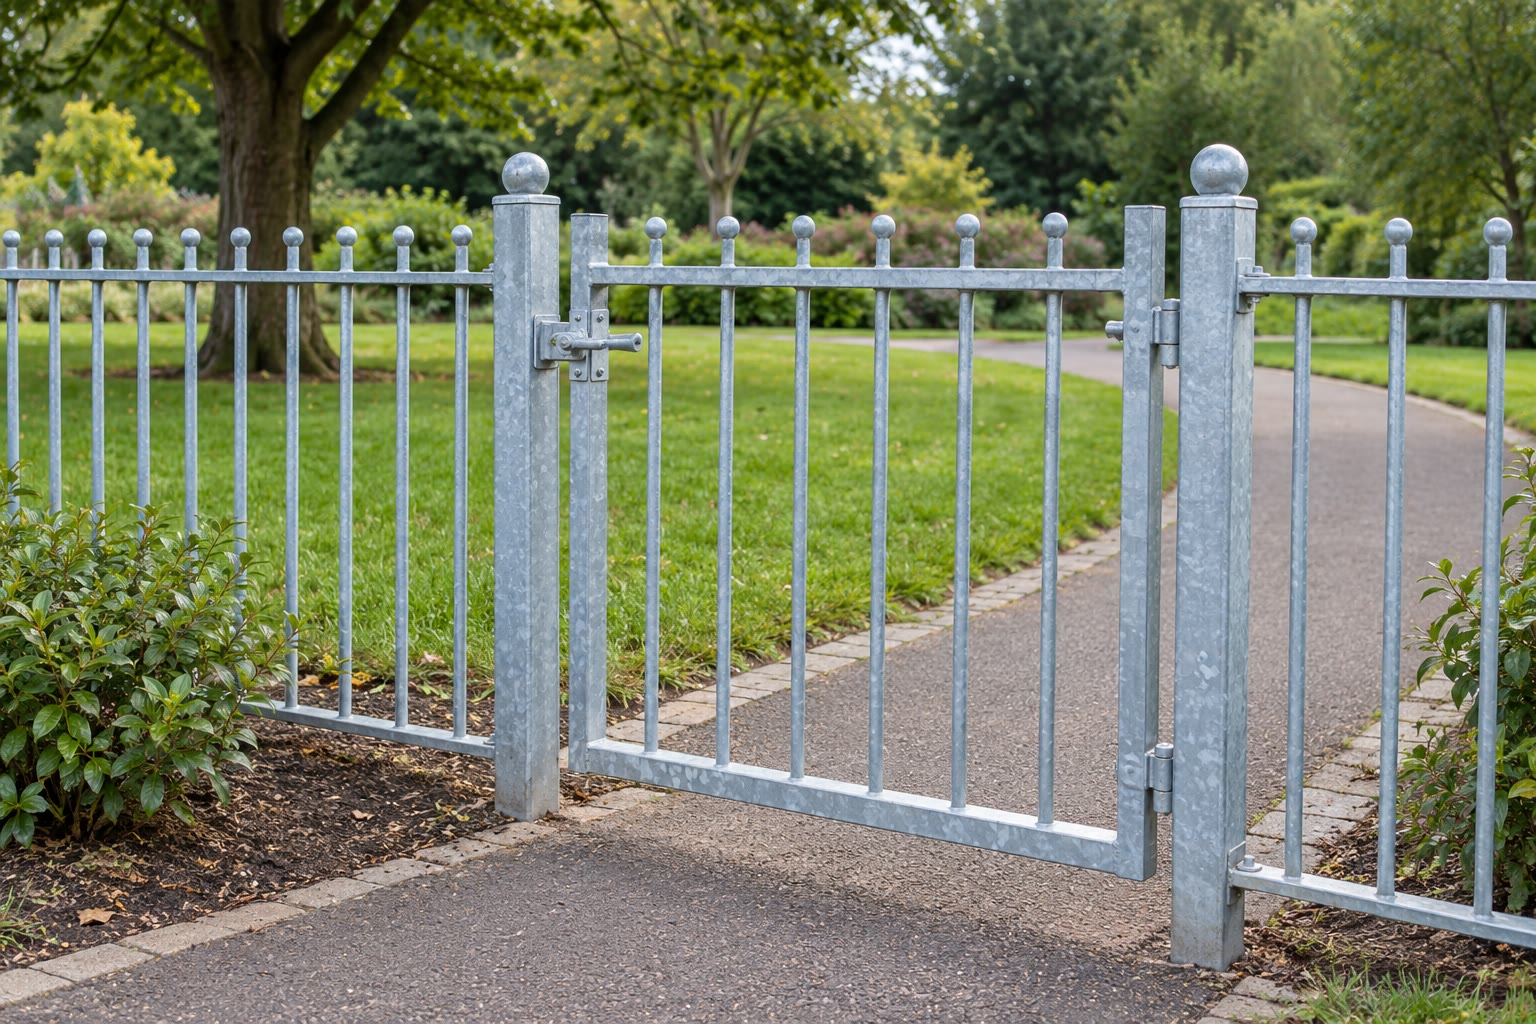
\includegraphics[width=\linewidth,height=4.4cm,keepaspectratio]{images/book1/ai/g9-galvanised-railings.jpg}

{\small Pagar baja berlapis seng.}
\end{minipage}
\end{omfigure}

\section{Latihan}

\begin{exercise}[$\star$]\label{exo:g9:metals-acids-corrosion:1}
Gas apa yang dilepaskan ketika seng bereaksi dengan asam klorida?
Bagaimana gas itu dikenali?
\end{exercise}

\begin{exercise}[$\star$]\label{exo:g9:metals-acids-corrosion:2}
Manakah di antara logam-logam berikut yang bereaksi dengan asam klorida
encer: besi, tembaga, seng, emas, aluminium?
\end{exercise}

\begin{exercise}[$\star$]\label{exo:g9:metals-acids-corrosion:3}
Apa yang diperlukan besi agar berkarat?
\end{exercise}

\begin{exercise}[$\star$]\label{exo:g9:metals-acids-corrosion:4}
Apa itu \omterm{def:g9:metals-acids-corrosion:spectator}{ion penonton}? Sebutkan \omterm{def:g9:metals-acids-corrosion:spectator}{ion penontonnya} ketika besi bereaksi
dengan asam klorida.
\end{exercise}

\begin{exercise}[$\star\star$]\label{exo:g9:metals-acids-corrosion:5}
Tuliskan \omterm{def:g8:balanced-equations:equation}{persamaan reaksi} magnesium dengan \omterm{def:g9:ions:ion}{ion-ion} \ce{H+} sebuah asam
(\omterm{def:g9:ions:ion}{ion} magnesium adalah \ce{Mg^{2+}}). Periksalah muatannya.
\end{exercise}

\begin{exercise}[$\star\star$]\label{exo:g9:metals-acids-corrosion:6}
Setelah besi bereaksi dengan asam klorida, bagaimana kamu dapat
menunjukkan bahwa larutannya mengandung \omterm{def:g9:ions:ion}{ion} besi(II)?
\end{exercise}

\begin{exercise}[$\star\star$]\label{exo:g9:metals-acids-corrosion:7}
Lihatlah gambar tiga paku. Mengapa air dalam tabung kedua dididihkan
dan ditutup minyak?
\end{exercise}

\begin{exercise}[$\star\star$]\label{exo:g9:metals-acids-corrosion:8}
Mengapa mobil lebih cepat berkarat di kota yang jalan-jalannya ditaburi
garam pada musim dingin?
\end{exercise}

\begin{exercise}[$\star\star$]\label{exo:g9:metals-acids-corrosion:9}
Mengapa kusen jendela aluminium tidak habis berkarat, padahal aluminium
bereaksi dengan oksigen \omterm{def:g4:air-a-mixture-of-gases:air}{udara}?
\end{exercise}

\begin{exercise}[$\star\star$]\label{exo:g9:metals-acids-corrosion:10}
Berikan tiga cara melindungi rangka sepeda dari baja terhadap \omterm{def:g9:metals-acids-corrosion:corrosion}{karat}.
\end{exercise}

\begin{exercise}[$\star\star\star$]\label{exo:g9:metals-acids-corrosion:11}
Tuliskan dan periksalah \omterm{def:g8:balanced-equations:equation}{persamaan reaksi} aluminium dengan \omterm{def:g9:ions:ion}{ion-ion}
\ce{H+} sebuah asam. Berapa \omterm{def:g7:atoms-and-molecules:molecule}{molekul} hidrogen yang terbentuk untuk 200
\omterm{def:g7:atoms-and-molecules:atom}{atom} aluminium?
\end{exercise}

\begin{exercise}[$\star\star\star$]\label{exo:g9:metals-acids-corrosion:12}
Sebuah ember baja berlapis seng tergores sampai ke bajanya. Jelaskan
mengapa baja di dasar goresan itu tidak berkarat untuk waktu yang lama.
\end{exercise}

\section{Soal: Berapa Tebal Lapisan Sengnya?}

\begin{problem}[{Soal akhir pekan --- melarutkan lapisan seng sebuah pelat
berlapis seng untuk mengetahui tebalnya}]
\label{pb:g9:metals-acids-corrosion:1}
% ledger: rho:Zn
Sebuah pelat baja berlapis seng, berbentuk persegi bersisi
\qty{10.0}{cm}, dilapisi seng pada kedua permukaannya (tepi-tepinya
diabaikan). Di laboratorium, guru menimbangnya, \qty{125.6}{g}, lalu
mencelupkannya ke dalam asam klorida yang mengandung zat tambahan yang
mencegah asam menyerang baja. Ketika gelembung-gelembungnya berhenti,
pelat itu dibilas, dikeringkan, dan ditimbang lagi: \qty{113.5}{g}.
Massa \qty{1}{cm^3} seng adalah \qty{7.13}{g}.

\medskip
\noindent\textbf{Bagian I --- Reaksinya.}
\begin{enumerate}
  \item Tuliskan \omterm{def:g8:balanced-equations:equation}{persamaan reaksi} seng dengan \omterm{def:g9:ions:ion}{ion-ion} \ce{H+} dari asam.
  \item Gas apa yang menimbulkan gelembung? Uraikan ujinya.
  \item Uji apa yang akan menunjukkan \omterm{def:g9:ions:ion}{ion-ion} seng di dalam larutan
        sesudahnya?
  \item Sebutkan \omterm{def:g9:ions:ion}{ion-ion} penontonnya.
\end{enumerate}

\medskip
\noindent\textbf{Bagian II --- Sengnya.}
\begin{enumerate}[resume]
  \item Berapa massa seng yang telah \omterm{def:g2:mixing-and-dissolving:dissolve}{larut}?
  \item Mengapa gelembung-gelembung itu menjadi tanda bahwa sengnya belum
        \omterm{def:g2:mixing-and-dissolving:dissolve}{larut} seluruhnya?
  \item Apa yang akan terjadi pada baja jika asam itu tidak mengandung
        zat tambahan? Uji apa yang kemudian akan menunjukkannya?
  \item Mengapa seng melindungi baja pada pelat itu selama seng itu masih
        ada?
\end{enumerate}

\medskip
\noindent\textbf{Bagian III --- Tebalnya.}
\begin{enumerate}[resume]
  \item Berapa luas total permukaan pelat yang dilapisi, dalam
        \unit{cm^2}?
  \item Berapa volume yang ditempati seng itu?
  \item Simpulkan tebal lapisan seng itu, dalam sentimeter.
  \item Nyatakan tebal itu dalam mikrometer
        (\qty{1}{cm} $= \qty{10000}{\micro m}$).
\end{enumerate}
\end{problem}
